\section{Introduction to Neural Networks}
\subsection{Fundamental Structure}
\begin{flushleft}
    \large {To understand deep learning (DL) on a deeper level, we must first look closer at neural networks. They are ubiquitous in the space of DL and are the backbone or an integral part of most modern DL model architectures. As such, understanding what they are and where their ``power'' comes from is very important for both reasoning about the capabilities of DL systems and designing your own. \break
    
    Neural networks are learning algorithms loosely modeled after the brain. We will expand on this connection further in the future, but for now here are the basics: \textbf{Neurons} in the brain have lots of connections to other neurons, and can pass information between each other using electrical potentials shot down a long section of the cell called an \textbf{axon}. We \textit{heavily} abstract this complex biological process by representing it as a directed graph. We represent the neurons as nodes, and the axons as edges. \break
    
    The figure below shows how a graph like this might appear.}
    \begin{figure}[H]
        \centering
        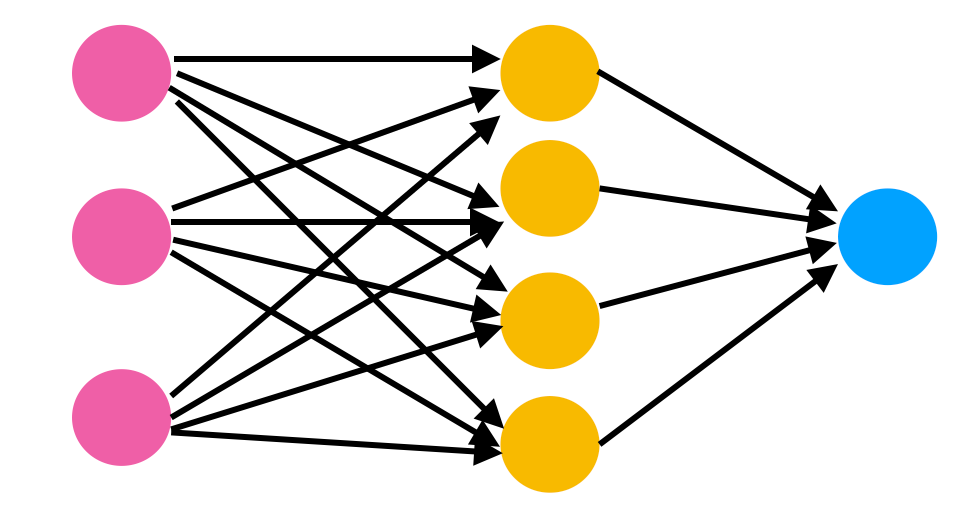
\includegraphics[width=0.5\linewidth]{dl/neuralnetwork.png}
        \caption{A visualization of neural networks}
        \label{fig:neuralnetwork}
    \end{figure}
\end{flushleft}

    \begin{flushleft}
    \large {As you can see in Figure 1 above, there are different levels or layers of neurons (pink, then yellow, and finally blue). That is a key characteristic of deep learning, a learning algorithm that uses \textbf{hierarchical layers to process information}. \break
    
    The primary layer of neurons is called the \textbf{input layer} - this is the layer where our input is read in as a vector. So if, for example, our input was an image (which is common as deep learning algorithms are often used for image classification), the image would be reconfigured into a large single-column vector, where each entry would represent a pixel in the image. The image would be, technically, entered into the model as one long vector of pixels, and this vector would be entered into the input layer of the model.}
    \end{flushleft}

\begin{figure}[H]
    \centering
    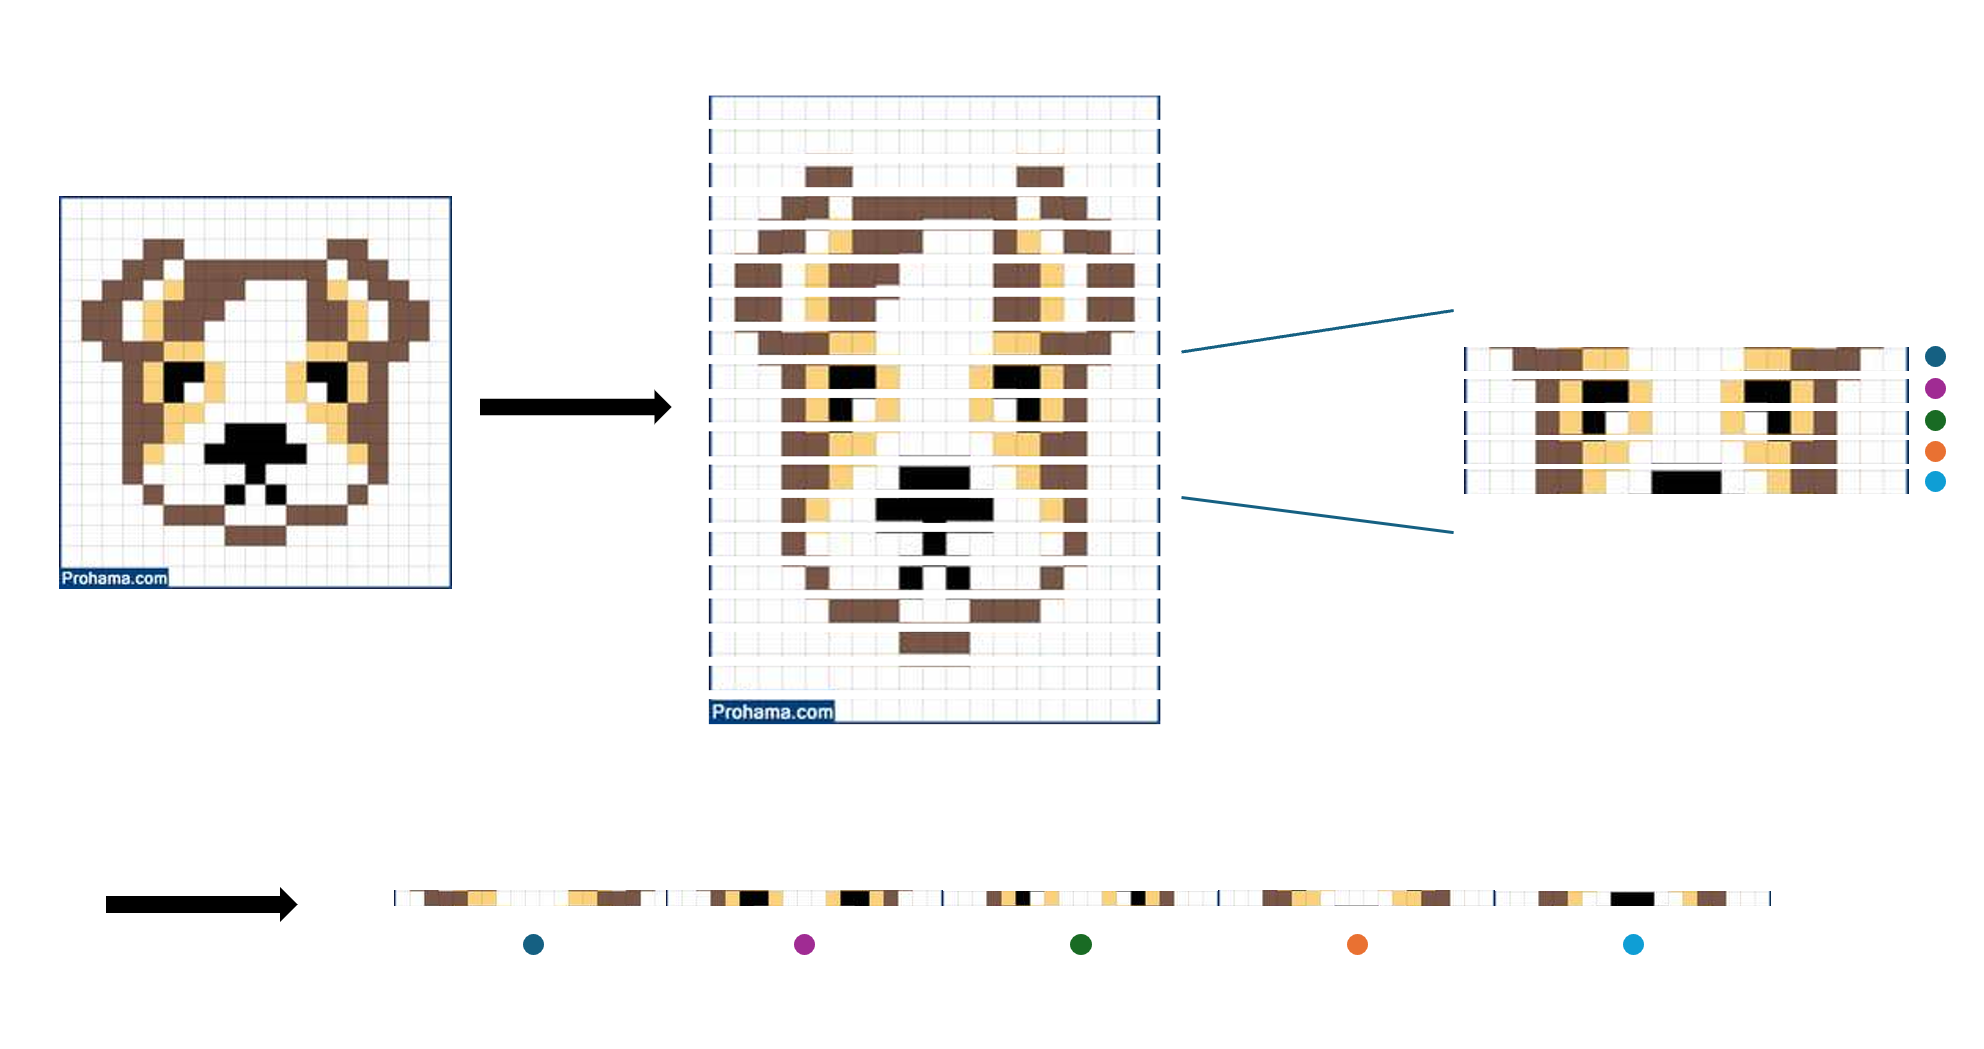
\includegraphics[width=1\linewidth]{dl/img-vector.png}
    \caption{Visualization of how images are converted into vectors}
    \label{fig:img-vector}
\end{figure}

\begin{flushleft}
    \large {Next are the \textbf{hidden layers}, which are yellow in the first image. There are usually multiple hidden layers in deep learning models, depending on how much processing the model must do before it can make a conclusion. The hidden layers are called ``hidden'' because we often don't understand what happens in here. Trying to interpret the vectors that exist in these layers usually results in nonsense. The field of explainable AI (XAI) has done lots of work here and there do exist tools to probe the hidden layers to understand what the model is ``thinking'' (I use the term thinking \textit{very} loosely here). However, without these tools, the middle of the network is considered a ``black box'' - a term you may have come across before. \break
    
    Finally, the \textbf{output layer}. The neural network calculates a probability for each possible outcome (for example, the input being an image of a dog) and fills out the output layer with values (blue in Figure 1). The output layer shows the algorithm's conclusions for the probabilities of each possible outcome and using these probabilities, the computer chooses an outcome. For classification neural networks, all the probabilities in the outcome layer will always add up to 1. Since there is one probability calculated for each outcome, the number of nodes in the output layer will be the number of possible outcomes. \break
    
    A small aside: Image inputs are the most common introduction to neural networks, because the ``Hello World'' project of deep learning, or the most introductory deep learning project, concerns image classification. It is important to note, however, that we could instead input ``features'' of some object we wish to classify or regress on. For example, we could provide the neural network with a vector consisting of the first index being the number of legs of an animal, the second index the height, the third a boolean indicating if it is a carnivore, etc. So, why don't we? \break
    
    A large reason neural networks are so useful is that they don't require too much ``feature engineering'' to get good results. Before the proliferation of the neural network, people would write complex algorithms to extract some features from an image. Where and how large the eyes of an animal are, an estimated number of legs, its edge contours, and many more complex features. They would then feed these vectors into a more traditional classification algorithm like a decision tree. \textbf{Neural networks are powerful enough that we can just cut up the raw image and throw it in. No complex engineering required!} This is why images are used in beginner projects: to demonstrate the power of these networks. However, this comes at the cost of efficiency. Neural networks often require orders of magnitude more data to train on, and also a lot more compute. The reasons for this will be explained in later sections.}
\end{flushleft}
\subsection{Flow of Information}
\begin{flushleft}
    \large Now that you understand the different layers of a neural network, let's see how the values in the input layer travel through the edges to get to the output layer. For ease of understanding, we are using a very simplified and weak version of a neural network, which we will improve in later sections. \break
    
    \textbf{Weights:} Zoom in one of the neurons in the input layer, and see how it connects to the next hidden layer. You will see one arrow pointing to each of the yellow neurons. Each of these arrows has a number attached to it. We call these numbers ``weights'' because they determine how much information from the previous node enters the next node. If you have a node with value $a$ connected to node $z$ with weight $w$, Node $z$ takes on the value of $a$ times $w$. If $w$ is very large or small, then this will heavily influence the value in $z$. If $w$ is closer to 0, then $z$ will not be influenced much by the value in $a$. You will also notice that one yellow neuron has multiple arrows going into it. This means multiple different neurons in the previous layer are sending their information over to this one. you just sum up the contributions. Nothing fancy there! \break
    
    \textbf{Biases:} Each neuron has a ``bias'' term that is added to its value. It can be positive or negative and make the neuron more ``sensitive'' to input. For example, a bias of +5 means that even if the values coming in from the previous layer to this neuron are generally negative, it is counteracted with a positive bias. Vice versa for negative biases. \break
    
    Let's write this all out: \break
    
    Have the three pink neurons be $a_1$, $a_2$, $a_3$. Only consider the top yellow neuron, and call it $z$. The arrow connecting $a_x$ to $z$ is called $w_x$. The bias for the neuron $z$ is $b$. 

    \begin{figure}[H]
        \centering
        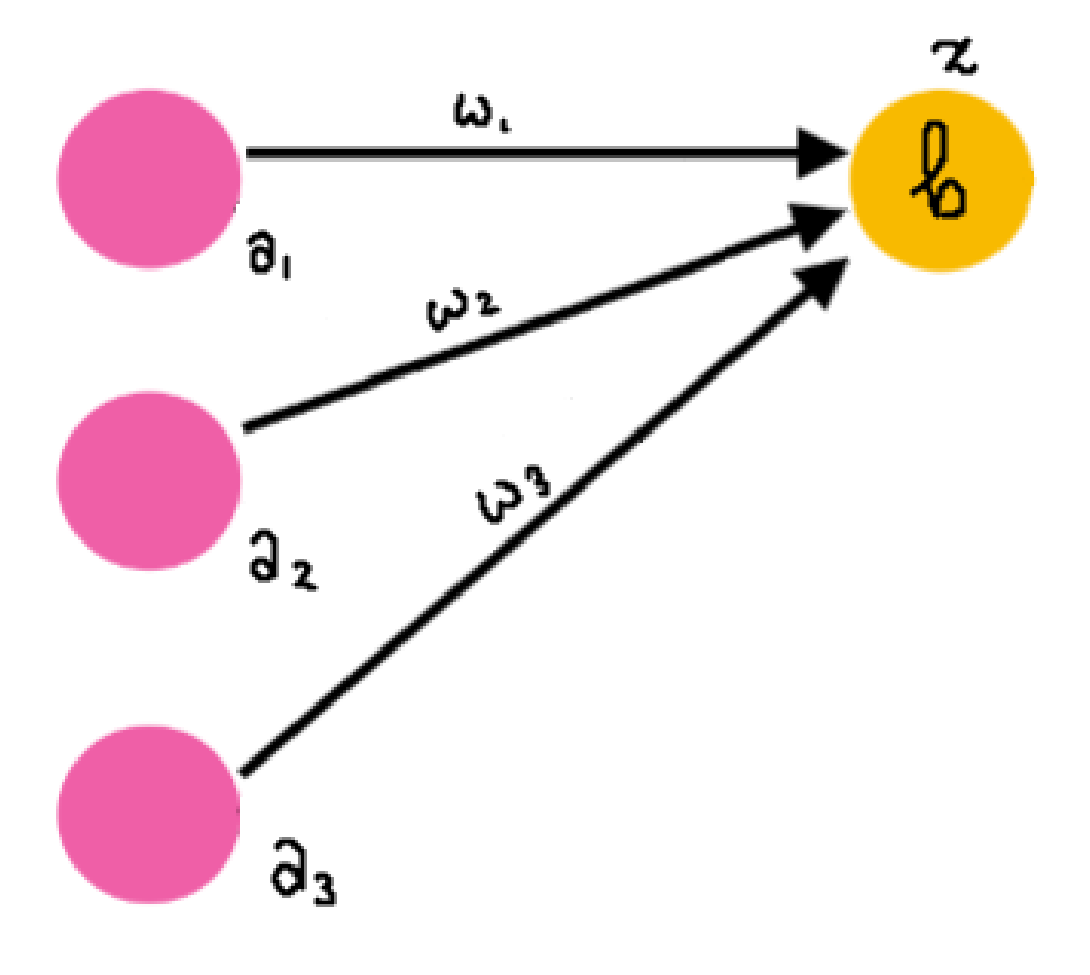
\includegraphics[width=0.5\linewidth]{dl/connectivity_basic.png}
        \caption{An illustration of weights and biases connecting the first layer of our neural network to the first neuron of the second (hidden) layer.}
        \label{fig:connectivity_basic}
    \end{figure}

    $$z = (w_1a_1 + w_2a_2 + w_3a_3) + b$$

    That is how information is propagated! This process is repeated for every neuron in the hidden layers, all the way out to the output layer. However, this is not done sequentially as shown above, but through the use of \textbf{matrices}.

    The \textbf{dot product} of two vectors of the same dimension $\textbf{a}$, $\textbf{b}$ is written as $\textbf{a} \cdot \textbf{b}$, and when expanded becomes:

    $$\sum_{i=1}^n a_ib_i$$

    Where $\textbf{a}$, $\textbf{b}$ $\in \mathbb{R}^n$. This is just saying that the vectors both have $n$ elements in them. We can rewrite the equation for $z$ as:

    $$z = \textbf{w}\cdot\textbf{a} + b$$

    We can add further subscripts to allow us to consider the whole hidden layer instead of one yellow neuron. Have the four yellow neurons be $z_1$, $z_2$, $z_3$, $z_4$. $\textbf{w}_x$ would then be a vector of the weights connecting the previous layer to $z_x$. We also add a subscript to the bias term to indicate which neuron in the hidden layer it belongs to. We now have, for the entire hidden layer:

    $$z_1 = \textbf{w}_1\cdot\textbf{a} + b_1$$
    $$z_2 = \textbf{w}_2\cdot\textbf{a} + b_2$$
    $$z_3 = \textbf{w}_3\cdot\textbf{a} + b_3$$
    $$z_4 = \textbf{w}_4\cdot\textbf{a} + b_4$$

    Using the properties of matrix multiplication (see \href{https://www.mathsisfun.com/algebra/matrix-multiplying.html}{here} if you need a refresher), we can simplify this further! We can define a \textbf{weight matrix} $W$ as a 4 $\times$ 3 matrix (4 rows, 3 columns):

    $$W = \begin{bmatrix}
            \textbf{w}_1\\
            \textbf{w}_2\\
            \textbf{w}_3\\
            \textbf{w}_4\\
            \end{bmatrix} = \begin{bmatrix}
                            w^1_1 & w^1_2 & w^1_3 \\
                            w^2_1 & w^2_2 & w^2_3 \\
                            w^3_1 & w^3_2 & w^3_3 \\
                            w^4_1 & w^4_2 & w^4_3 \\
                            \end{bmatrix}$$

    Making $\textbf{z}$ a vector holding all $z_x$ values and $\textbf{b}$ a vector holding all $b_x$ values, we can write:

    $$\textbf{z} = W\textbf{a} + \textbf{b}$$

    With the dimensions being: $\textbf{z} \in \mathbb{R}^{4 \times 1}$, $W \in \mathbb{R}^{4 \times 3}$, $\textbf{a} \in \mathbb{R}^{3 \times 1}$, and $\textbf{b} \in \mathbb{R}^{4 \times 1}$. Based on the architecture of your neural network, these numbers will change in expected ways.
\end{flushleft}

\subsection{The Perceptron and XOR}
\begin{flushleft}
    \large We just wrote out the equations that define how information flows between two layers in a neural network. Well, if we stop here and don't add any more layers, we come up with what is a \textbf{perceptron}. Understanding the limitations of two linear layers is crucial for appreciating the power of many nonlinear layers. Let us create a perceptron that accepts 2 inputs and outputs one.

    $$\textbf{z} = W\textbf{a} + \textbf{b}$$

    With the dimensions being: $\textbf{z} \in \mathbb{R}^{1 \times 1}$, $W \in \mathbb{R}^{1 \times 2}$, $\textbf{a} \in \mathbb{R}^{2 \times 1}$, and $\textbf{b} \in \mathbb{R}^{1 \times 1}$. Since the dimensions are so small, we can just do away with the compact matrix form:

    $$z = w_1a_1 + w_2a_2 + b$$

    $a_1$ and $a_2$ become $x$ and $y$ since we are in the Cartesian plane.

    $$z = w_1x + w_2y + b$$

    Subtract $b$:

    $$z - b = w_1x + w_2y$$

    Since $z$ and $b$ are constant, we have essentially written the standard form of a line! $w_1$, $w_2$, and $b$ define the line. Solving for $z$ tells you where the point $(x, y)$ lies in relation to the line. If $z$ is positive, the point lies above the line. 0 for on the line, and negative for below. \textbf{Therefore, the classification boundary a perceptron draws is linear.}

    What is this all for? Let's consider a famous problem: The XOR Problem. We construct a ``dataset'' from the definition of the XOR ($\oplus$) boolean function. The truth table for it can be seen below:

    $$\begin{array}{|c|c|c|}
    \hline
    X & Y & X \oplus Y \\
    \hline
    0 & 0 & 0 \\
    0 & 1 & 1 \\
    1 & 0 & 1 \\
    1 & 1 & 0 \\
    \hline
    \end{array}$$

    We can consider $X$ and $Y$ as Cartesian coordinates and $X \oplus Y$ as the ``class'' of the point. If this is plotted, you will quickly notice that \textit{there is no way to draw a line that cleanly separates the classes.} In other words, the XOR classification problem is \textbf{not linearly separable}.

    \begin{figure}[H]
        \centering
        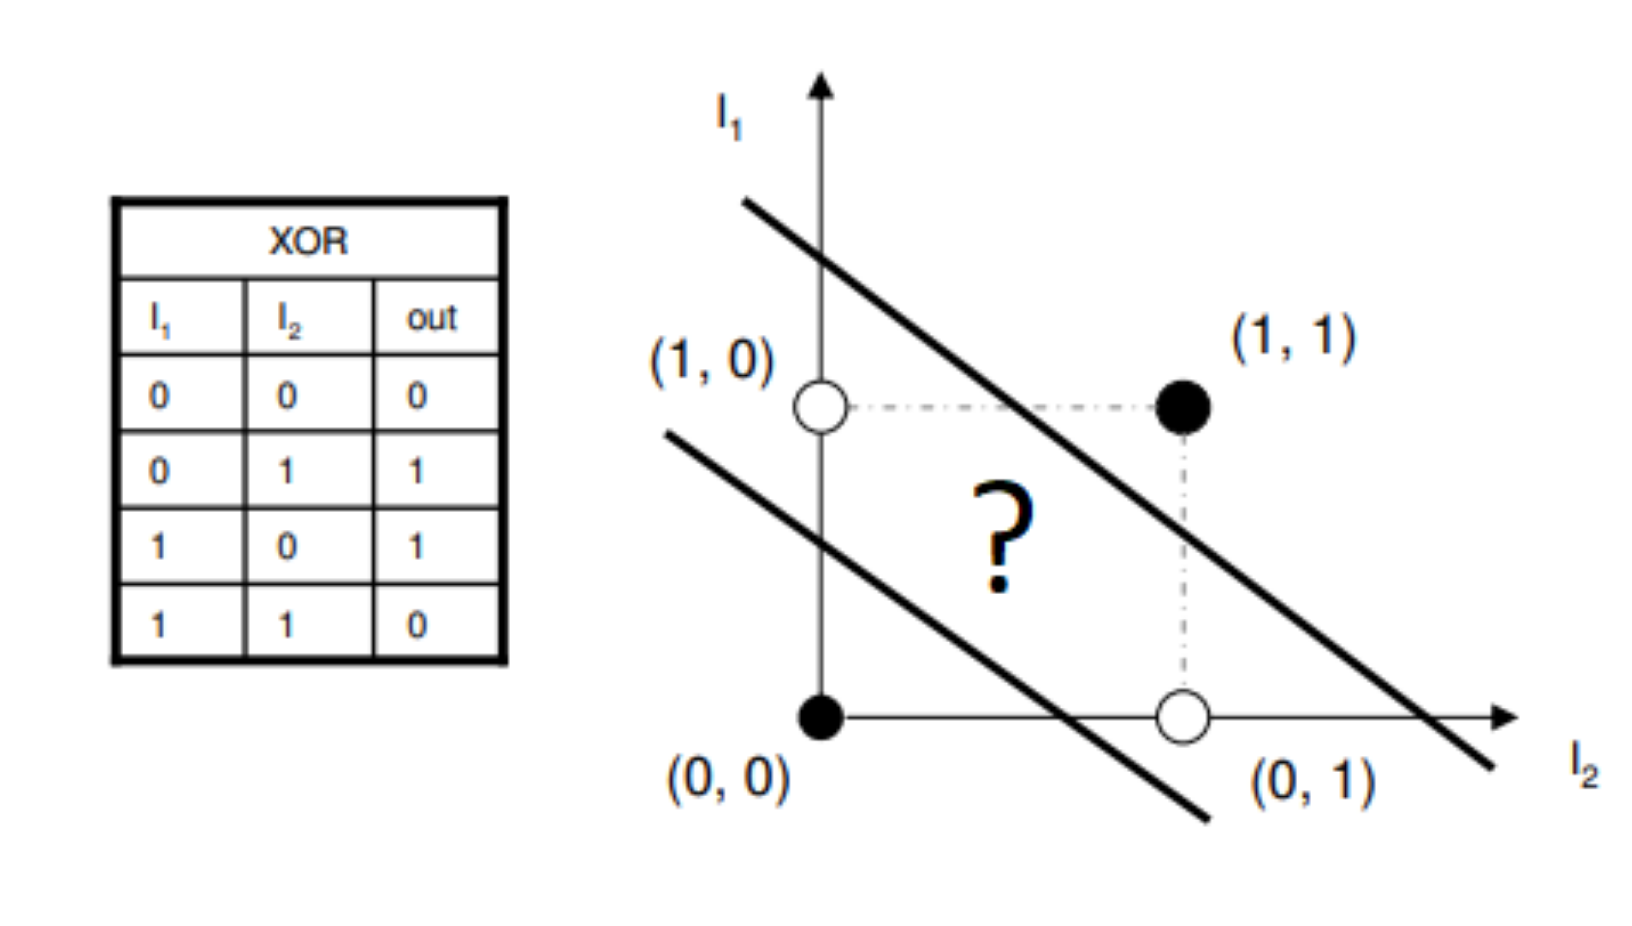
\includegraphics[width=0.5\linewidth]{dl/xor.png}
        \caption{Illustration of the XOR function, and how you cannot draw a single line that separates the classes (white and black dots).}
        \label{fig:xor}
    \end{figure}
    
    XOR is a simple boolean operation, as we move to complex problems like animal classification and speech recognition, how can perceptrons hope to solve them, even if we blow up the number of weights and nodes? You may say that we can add more layers, which can be represented as:

    $$\textbf{z}^1 = W^1\textbf{a} + \textbf{b}^1$$
    $$\textbf{z}^2 = W^2\textbf{z}^1 + \textbf{b}^2$$
    $$\textbf{z}^3 = W^3\textbf{z}^2 + \textbf{b}^3$$

    With superscripts just denoting what layer we are processing. Collapsing this set of equations through substitution:

    $$\textbf{z}^3 = W^3(W^2(W^1\textbf{a} + \textbf{b}^1) + \textbf{b}^2) + \textbf{b}^3$$

    Distribute:

    $$\textbf{z}^3 = W^3W^2W^1\textbf{a} + W^3W^2\textbf{b}^1 + W^3\textbf{b}^2 + \textbf{b}^3$$

    Here comes the issue with more layers. The term $W^3W^2W^1\textbf{a}$ can simply be collapsed into a single transformation $W\textbf{a}$! The decision boundary is still linear, and can therefore never ``solve'' a problem that is not linearly separable. The terms $ W^3W^2\textbf{b}^1 + W^3\textbf{b}^2 + \textbf{b}^3$ do not change this fact. Applying multiple linear transformations to a vector is the same as applying the product of those transformations all at once. The associative property of matrix multiplication totally allows this, since

    $$(AB)C = A(BC)$$

    Here is another way of looking at the above equation. See how the matrices can collapse into one?

    $$\textbf{z}^3 = (((W^3W^2)W^1)\textbf{a}) + W^3W^2\textbf{b}^1 + W^3\textbf{b}^2 + \textbf{b}^3$$
    
    Therefore we are back at square one as we were with two layers, just with more bias terms... So how do we make it so that we can draw more than just lines in our spaces to solve the XOR problem? The answer lies with nonlinearities (shocker!).
\end{flushleft}

\begin{questionbox}
\textbf{Synthesis Questions:}
\begin{enumerate}
    \item Define the following words:
    \begin{itemize}
        \item Neuron
        \item Layer
        \item Hidden Layer
        \item Weight
        \item Bias
    \end{itemize}
    \item If you have a neural network with an input dimension of 3, a hidden dimension of 4, and an output dimension of 1, then what would:
    \begin{itemize}
        \item The dimension of $W$ between the input and hidden layers be?
        \item The dimension of $W$ between the hidden and output layer be?
        \item The dimension of $\textbf{b}$ for the hidden layer?
    \end{itemize}
    \item Explain in your own words why a linear classifier (like a perceptron) cannot be used to solve the XOR problem
\end{enumerate}
\end{questionbox}

\section{Non-Linearity and Activation Functions}
\subsection{Introducing Nonlinearities}
\begin{flushleft}
    \large Let's take a step up from the XOR problem and look at something arguably more complex: Image classification. Image classification, especially with categories as specific as `dog' or `cat', is very challenging. It requires a level of detail and processing that many machine learning algorithms cannot achieve, especially linear algorithms, where a change in the input is directly proportional to the corresponding change in output. So, to tackle complex tasks such as image classification, neural networks, and deep learning models need to employ \textbf{non-linearity}. In non-linear models, changes in input can cause varying levels of change in corresponding output. Going back to our dog example, if we change the size of a dog's ear, we want that to have little impact on the model's conclusion. But if we change how the dog's fur appears, that should have a much larger impact. Non-linearity can help us achieve this. To introduce non-linearity to neural networks, models implement \textbf{activation functions}. \break
    
    Activation functions are applied after computing the raw values to populate the nodes of a neural network layer. These raw outputs are called \textbf{logits}. Recall Figure \ref{fig:neuralnetwork}. In the below equation, the values in the vector $\textbf{z}$ would be the logits of the hidden layer:

    $$\textbf{z} = W\textbf{a} + \textbf{b}$$

    This is NOT immediately what is passed to the final layer. Instead, we first apply a non-linear function to the logits. We can refer to this function as $\phi(\cdot)$, and we will give specific examples of this function later. Therefore, a multi-layer neural network (or in other words, a non-linear multi-layer perceptron) can be written out as follows:

    $$\textbf{z}^1 = \phi(W^1\textbf{a} + \textbf{b}^1)$$
    $$\textbf{z}^2 = \phi(W^2\textbf{z}^1 + \textbf{b}^2)$$
    $$\textbf{z}^3 = \phi(W^3\textbf{z}^2 + \textbf{b}^3)$$

    Now let's collapse this equation, and see if we run into the same problem we had with a multi-layer linear perceptron:

    $$\textbf{z}^3 = \phi(W^3\phi(W^2(\phi(W^1\textbf{a} + \textbf{b}^1) + \textbf{b}^2) + \textbf{b}^3)$$

    The matrices can no longer be collapsed into just one, meaning that we can \textit{draw more complex boundaries between classes, or find more complex patterns within regression tasks.} Using activation functions to allow for non-linearity gives deep learning and neural network models the strength to find solutions for complex tasks. A fundamental concept in the theory of neural networks, called the \textbf{Universal Approximation Theorem}, states that a neural network with at least one hidden layer with a finite number of neurons can approximate any continuous function to any level of accuracy with the use of certain activation functions. So, using non-linearity, neural networks can predict almost anything and do so accurately. Of course, we would also need enough data and compute to train this arbitrarily large model. \break
\end{flushleft}
\subsection{Common Activation Functions}

\begin{flushleft}
\begin{figure}[H]
    \centering
    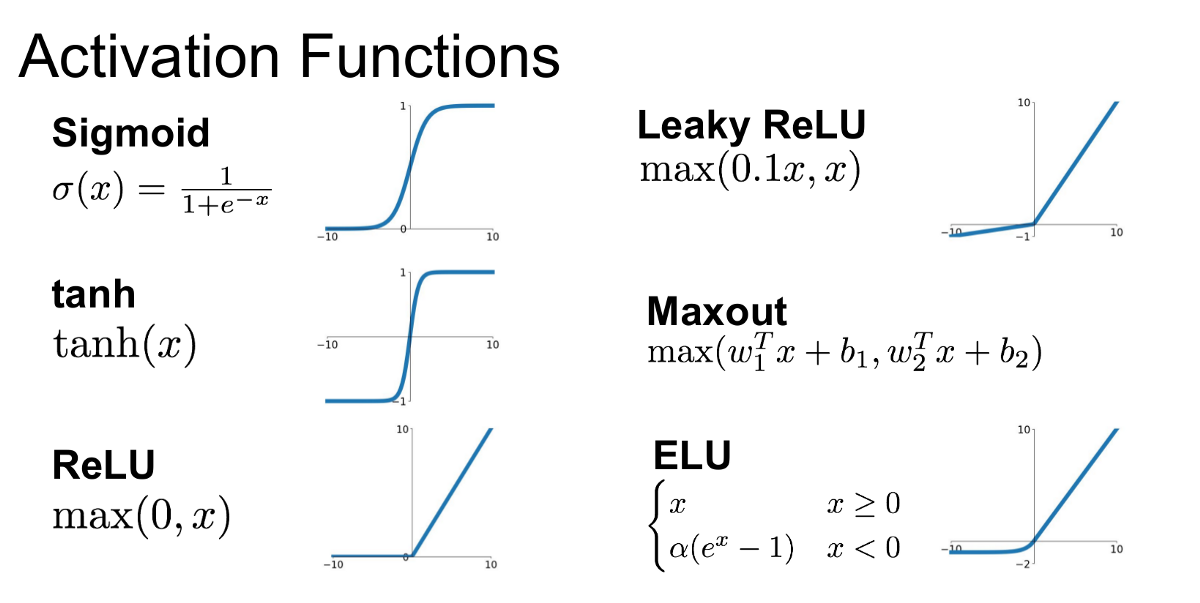
\includegraphics[width=0.75\linewidth]{dl/activationfuncs.png}
    \caption{Plots of various activation functions}
    \label{fig:activationfuncs}
\end{figure}
    \large One commonly used activation function is the \textbf{sigmoid function}. This function squashes inputs into the range between 0 and 1. It is useful in binary classification tasks but can cause issues like vanishing gradients in deeper networks (more on this later). The formula, where $x$ is a given neuron's output is:
    \begin{center}$\sigma(x) = \frac{1}{1+e^{-x}}$\end{center}
    The hyperbolic tangent activation function, or \textbf{tanh}, squashes inputs between -1 and 1. It is zero-centered, which makes it easier for optimization compared to the sigmoid function. The tanh formula is:
    \begin{center}$tanh(x) = \frac{e^x-e^{-x}}{e^x+e^{-x}}$\end{center}
    Another activation function, \textbf{Rectified Linear Unit or ReLU}, outputs the input if it's positive, and zero otherwise. It is computationally efficient and helps alleviate the vanishing gradient problem by allowing gradients to flow when the input is positive. ReLU is written as:
    \begin{center}$ReLU(x) = MAX(0,x)$\end{center}
    There is also another form of the ReLU activation function called \textbf{Leaky ReLU} that allows a small, non-zero gradient when the input is negative, helping prevent the issue of "dead neurons" (neurons that never activate). Leaky ReLU looks like:
    \begin{center}\[f(x)= 
        \begin{cases}
            x,& \text{if } x > 0\\
            0.01x,              & \text{if } x \leq 0
        \end{cases}
    \]\end{center}
\end{flushleft}

\begin{questionbox}
    \textbf{Synthesis Questions:}
    \begin{enumerate}
        \item Define the following words:
        \begin{itemize}
            \item Activation function
            \item Logits
        \end{itemize}
        \item Why are activation functions important for increasing the power of a neural network?
        \item In your own words, what is the Universal Approximation Theorem?
    \end{enumerate}
\end{questionbox}

\section{Backpropagation}
\subsection{Loss Functions}
\begin{flushleft}
    \large How does a neural network `learn' using training (a.k.a labeled) data? It uses a process called \textbf{backpropagation}. This process adjusts the weights assigned to connections between neurons and the biases assigned to nodes to improve the algorithm's accuracy. Imagine for a moment, that we are working with deep neural network classifying images as dog or cat. In this case, we will want to assign a higher weight to the feature `long tongue' because that is an important feature in determining whether something is a dog or a cat. To implement this functionality, the model will have a hidden neuron that ``lights up'' (has a high value) when the input animal image has a long tongue. This will significantly sway the model's decision-making process, increasing the probability of the image being a dog. In comparison, a neuron relating to the feature `fur color' might want to have a smaller weight connecting it to the next layer, because cats and dogs have similar fur colors and this feature isn't as important in differentiating between cats and dogs. The backpropagation process will slowly adjust these weights to be this way, leading to an excellent classifier. \break
    
    So how does backpropagation determine which weights and biases to manipulate? To understand that, we have to discuss \textbf{loss functions}. A loss function is used to measure how far off the network's predictions are from the actual target values. It provides a numeric value that represents the error in the prediction. Generally, higher loss means the model did not perform well, and vice versa. The goal of backpropagation is to reduce this loss by adjusting the weights in the network. A common example of a loss function is \textbf{Mean Squared Error (MSE)}, which is often used for regression tasks. The formula for MSE is:
    
    $$L = \frac{1}{N} \sum^{N}_{i=1} (y_i - \hat{y}_i)^2$$
    
    where $L$ is the loss, or the model's error, $y_i$ is the target-value (also known as the correct answer or label) for the specific input, $\hat{y}_i$ is the value the model predicted/guessed, and $N$ is the number of training examples shown to the model. You may notice that this version of the MSE loss function works only with scalar outputs from a neural network. There are versions of MSE that can handle multiclass output. However, it is generally accepted that if you have a multiclass classification problem, a better loss function to use is \textbf{Cross-Entropy Loss} (or log loss). This loss function measures the difference between two probability distributions. The formula for Cross-Entropy Loss is: 
    
    $$ L = -\frac{1}{N}\sum^{N}_{i=1} \sum^{K}_{k=1} y_{ik} \cdot log(\hat{y}_{ik})$$
    
    where $K$ is one of the outcomes or classes, $y_i$ is the actual probability of the given input belonging in class $K$, and $\hat{y}_i$ is the probability the model has assigned to class $K$ for the given input. \break
    
    Calculating these loss metrics is the final step of what is called the \textbf{forward pass}. This is what we have studied so far. After this begins the \textbf{backward pass} or \textbf{backpropagation}. 
\end{flushleft}

\subsection{Derivatives and Gradients}
\begin{flushleft}
    \large Before we delve into the semi-convoluted math behind backpropagation, we should revisit some concepts from calculus. Take a look at the equation and associated graph below:

    $$f(x, y) = z = x^2 + y^2$$

    \begin{figure}[H]
        \centering
        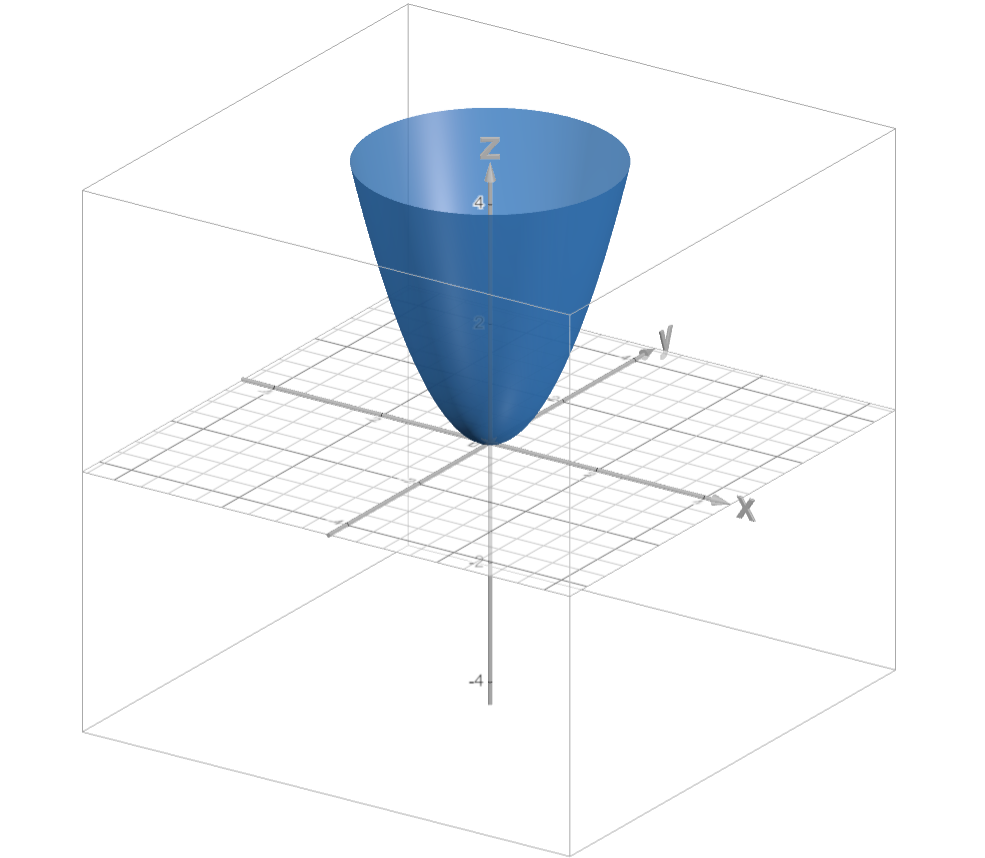
\includegraphics[width=0.5\linewidth]{dl/x2y2.png}
        \caption{Illustration of the function $f(x, y) = x^2 + y^2$}
        \label{fig:x2y2}
    \end{figure}

    The \textbf{gradient} of a multivariate function (denoted in this case as $\nabla f(x,y)$ or $\nabla z$) points you in the \textit{direction of steepest ascent} of a function given a point. To calculate the gradient of a function, you simply take the partial derivative of the function with respect to each variable and represent the derivatives as directions of a vector. Here is an example using $f(x,y) = z = x^2 + y^2$:

    $$\nabla z = \begin{bmatrix}
            \frac{\partial z}{\partial x}\\
            \frac{\partial z}{\partial y}\\
            \end{bmatrix}$$

    Solve for $\frac{\partial z}{\partial x}$:

    $$\frac{\partial}{\partial x}z = \frac{\partial}{\partial x}(x^2 + y^2)$$
    $$\frac{\partial z}{\partial x} = 2x$$

    Solve for $\frac{\partial z}{\partial y}$:
    
    $$\frac{\partial}{\partial y}z = \frac{\partial}{\partial y}(x^2 + y^2)$$
    $$\frac{\partial z}{\partial y} = yx$$

    $$\nabla z = \begin{bmatrix}
            2x\\
            2y\\
            \end{bmatrix}$$

    We now have a way to, given any point on the function, determine which direction to move to increase $z$ the most. If we plug in $(1,1)$, we get 
    
    $$\begin{bmatrix}
            2\\
            2\\
    \end{bmatrix}$$

    If we plot this as a vector on our previous graph:

    \begin{figure}[H]
        \centering
        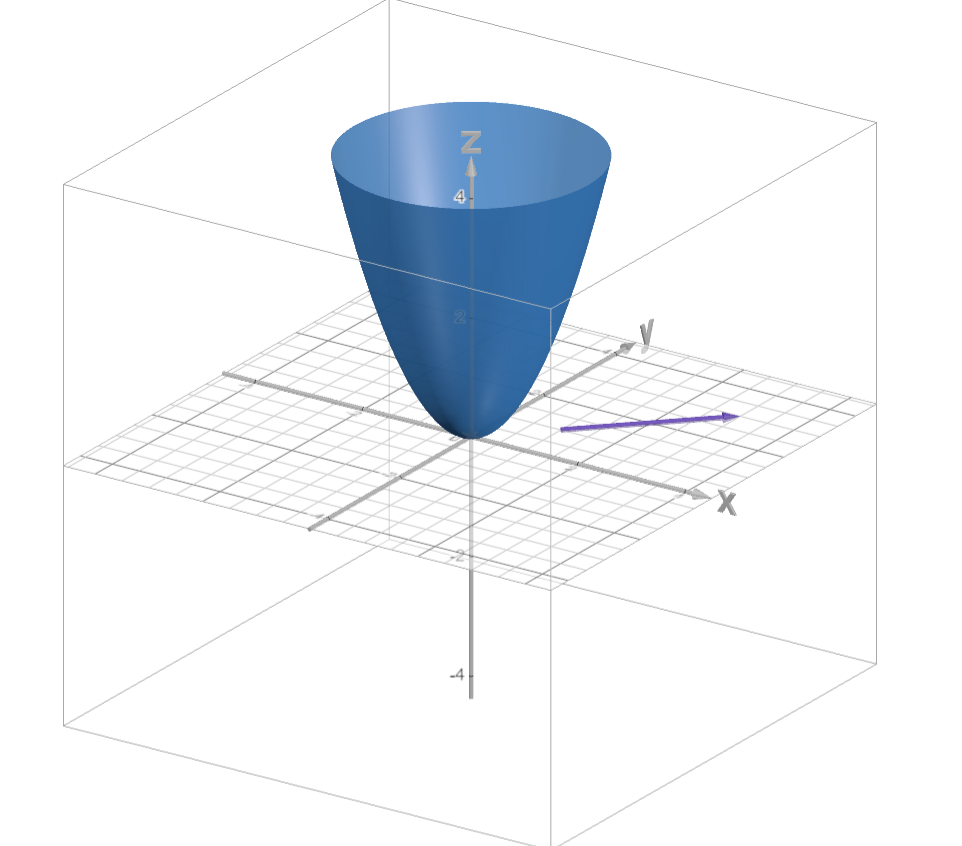
\includegraphics[width=0.45\linewidth]{dl/x2y2line.png}
        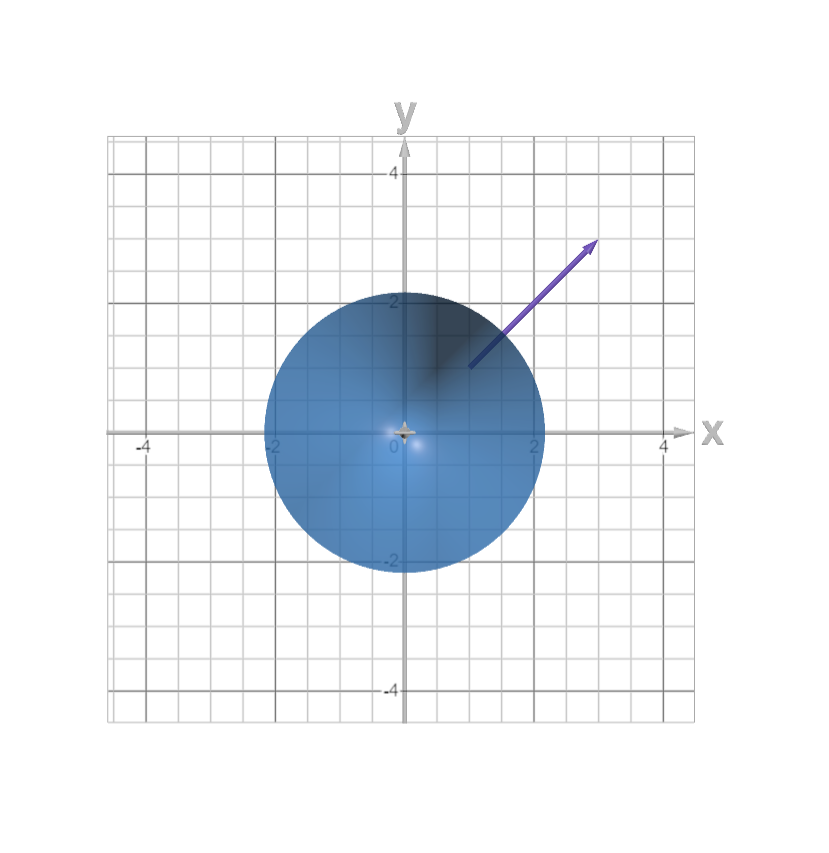
\includegraphics[width=0.45\linewidth]{dl/x2y2lineabove.png}
        \caption{Illustration of the function $f(x, y) = x^2 + y^2$, with a vector showing the direction of steepest ascent from point $(1,1)$}
        \label{fig:x2y2_2}
    \end{figure}

    So how does this relate to neural networks? Well, we can simply think of a neural network as a large multivariate function, with the variables in question being the weights. Think about it: we have a loss function that we want to reduce. We can imagine this as $z$ in the previous example. We want to find out how to change the weights to \textit{reduce} the loss function the quickest (direction of steepest descent). So, we just flip the idea of a gradient on its head. If we can find $\nabla_W L$ (the gradient of $L$ with respect to all weights), we can adjust the weights to minimize the loss!

    $$W_{new} \leftarrow W_{old} - \nabla_W L$$

    Calculating this by hand is near impossible, and nobody expects you to. There are tricks we can use to calculate gradients in chunks rather than taking 100's of derivatives.
\end{flushleft}

\subsection{Gradient Flow}
\begin{flushleft}
    \large The model first calculates the derivative of the loss with respect to $\hat{y}_i$, since $\hat{y}_i$ is the output of the model. For ease of understanding, we will use MSE loss:

    $$L = \frac{1}{N} \sum^{N}_{i=1} (y_i - \hat{y}_i)^2$$
    $$\frac{\partial}{\partial \hat{y}} L = \frac{\partial}{\partial \hat{y}}  \frac{1}{N} \sum^{N}_{i=1} (y_i - \hat{y}_i)^2$$
    $$\frac{\partial L}{\partial \hat{y}} =  \frac{1}{N} \sum^{N}_{i=1} -2(y_i - \hat{y}_i)$$

    This value is directly calculable, and it is propagated backward, starting ``gradient flow''. \break

    Lets say $\hat{y_i} = \sigma(z)$. Recall that $\sigma(\cdot)$ represents the \textbf{sigmoid} activation function. This therefore represents the activation function applied to the logits of the output neuron. \break
    
    Also define $z = f(w_1, w_2, ... w_n) = \sum_{i=1}^n a_iw_i + b$. Recall that $a_i$ is the output of neuron $i$ from the previous layer. This therefore represents the calculation of the output neuron's logits using the outputs from the neurons of the previous layer. \break
    
    % This is all visually represented in the image below:

    % \begin{figure}[H]
    %     \centering
    %     \includegraphics[width=0.5\linewidth]{}
    %     \caption{\todo{Create this image}}
    %     \label{fig:backpropviz}
    % \end{figure}

    How can we calculate $\nabla_W L = \biggl[ \frac{\partial L}{\partial w_1}, \frac{\partial L}{\partial w_2},...,  \frac{\partial L}{\partial w_n}\biggr]$? Using the chain rule, we can rewrite any $\frac{\partial L}{\partial w_x}$ as:

    $$\frac{\partial L}{\partial w_x} = \frac{\partial L}{\partial \hat{y}}\cdot\frac{\partial \hat{y}}{\partial z}\cdot\frac{\partial z}{\partial w_x}$$
    
    where $\frac{\partial L}{\partial w_x}$ is the gradient of the loss with respect to an arbitrary weight $w_x$, $\frac{\partial L}{\partial\hat{y}}$ is the gradient of the loss with respect to the predicted output, $\frac{\partial\hat{y}}{\partial z}$ is the gradient of the output with respect to the weighted sum $z$, and $\frac{\partial z}{\partial w}$ is the gradient of the weighted sum with respect to the weight $w$. \break

    We already have $\frac{\partial L}{\partial\hat{y}}$ as shown above. $\frac{\partial \hat{y}}{\partial z}$ is calculated as such:

    $$\hat{y_i} = \sigma(z)$$
    $$\frac{\partial}{\partial z}\hat{y_i} = \frac{\partial}{\partial z} \sigma(z)$$
    $$\frac{\partial \hat{y_i}}{\partial z} = \sigma'(z)$$

    $\sigma'(z)$ is just the derivative of the sigmoid. This is easy to compute. Calculating $\frac{\partial z}{\partial w_x}$ is a little harder, as we have considered $w_x$ as an arbitrary weight. Let us calculate the partial derivative with respect to just $w_1$. Calculating the other $w$ follows easily. \break

    $$f(w_1, w_2,...,w_n) = z = \sum_{i=1}^n a_iw_i + b$$
    $$\frac{\partial}{\partial w_1}z = \frac{\partial}{\partial w_1}\sum_{i=1}^n a_iw_i + b$$
    $$\frac{\partial z}{\partial w_1} = a_1$$

    It follows that $\frac{\partial z}{\partial w_2} = a_2$, $\frac{\partial z}{\partial w_3} = a_3$, and so forth. Therefore we can say that $\frac{\partial z}{\partial w_x} = a_x$. We can plug all these results into our chain rule:

    $$\frac{\partial L}{\partial w_x} = \frac{\partial L}{\partial \hat{y}}\cdot\frac{\partial \hat{y}}{\partial z}\cdot\frac{\partial z}{\partial w_x}$$
    $$\frac{\partial L}{\partial w_x} =  (\frac{1}{N}\sum^{N}_{i=1} -2(y_i - \hat{y}_i)) \cdot (\sigma'(z)) \cdot (a_x)$$

    For deeper neural networks with many layers, this computational graph becomes much more complex. However, the idea stays the same: Find the gradients of the loss with respect to the weights of each layer. Do this by passing gradients backward through the network. Calculating the gradient with respect to the biases is done the same, and even simpler! Performing gradient descent is then as simple as the equation from before, with a small constant added to ensure these changes are incremental and not massive:

    $$W_{new} \leftarrow W_{old} - \lambda\nabla_W L$$

    This constant $\lambda$ is called the \textbf{learning rate}, and we will discuss its significance later. Congratulations, you know understand basic gradient descent!
\end{flushleft}

\subsection{Optimizers and Learning Rates}
\begin{flushleft}
    \large While gradient descent is a common optimizer and is easy to follow mathematically, it is unfortunately very expensive computationally and can be slow. \textbf{Stochastic Gradient Descent (SGD)} is a similar, more efficient, optimizer. SGD speeds up this process by updating weights after computing the gradient on a small, random batch of data, rather than the entire dataset. Another popular optimizer is \textbf{Adam}. Adam combines the benefits of both SGD and another optimization technique called \textbf{Momentum}, which helps the optimizer move faster by incorporating information from past gradients. Adam also adapts the learning rate for each weight based on how the gradients change, making it efficient for handling noisy gradients and sparse data. Many people use Adam because it performs well across a wide range of tasks. It is essential to understand that Adam fine-tunes the learning process dynamically, making it more flexible than standard SGD. A deep dive into how each of these optimizers work is a bit beyond the scope of this article, but is interesting and I suggest you do some independent research! \break
    
    A common thread between all of these optimizers is that they share one parameter in common: the \textbf{learning rate}. This is a scaling factor applied to the calculated gradient before it is used to adjust the weights. The size of this scaling determines how big of a ``step'' the weights take while traversing the ``loss landscape''. Optimizer classes in most deep learning libraries (e.g. PyTorch, Tensorflow) have defaults that work well for each of the different optimizers. Starting here is usually a good idea, because a learning rate that is too small will take way too long to converge, while a large learning rate may not converge at all! For an illustration of this, see Figure \ref{fig:lr}.

    \begin{figure}[H]
        \centering
        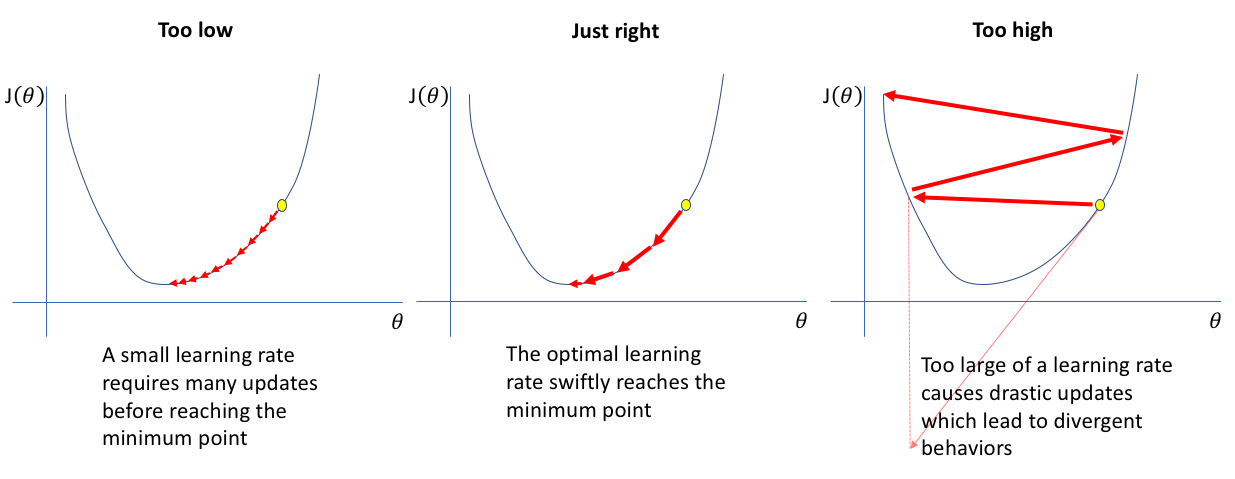
\includegraphics[width=1\linewidth]{dl/lr.png}
        \caption{A demonstration of how different learning rates affect convergence of a loss function (in this graphic represented as $J(\theta).$}
        \label{fig:lr}
    \end{figure}
\end{flushleft}

\begin{questionbox}
    \textbf{Synthesis Questions:}
    \begin{enumerate}
        \item Define what the purpose of a loss function is
        \item What are the different use cases for Mean Squared Error vs. Cross Entropy Loss?
        \item What is the difference between a derivative and a gradient?
        \item Find the gradient for this function at $(3, 2, 1)$:
        $$f(x,y,z) = \frac{2}{3}x^2 + y^2 - 2y + z^4 - \frac{4}{3}z^3$$
        \item Find the derivative of the sigmoid ($\sigma$) function and plot it. Why might this activation function prevent gradients from flowing back through the network during the backward pass?
        \item Why might the ``steps'' taken by SGD not be as directly in the most optimal direction compared to GD?
    \end{enumerate}
\end{questionbox}

\section{Regularization}
\begin{flushleft}
    \large We will now cover an incredibly important topic for deep learning: \textbf{regularization}. In ML, regularization often is applied in the form of adding a norm to the loss function, encouraging weights to reach smooth (L2) or sparse (L1) optima. Regularization also exists in deep learning to prevent overfitting, but comes about in more interesting and varied ways. We will quickly cover two common ones in shallow detail.
\end{flushleft}

\subsection{Dropout}
\begin{flushleft}
    \large \textbf{Dropout:} During each forward pass, a certain fraction of neurons are temporarily dropped from the neural network. The connections they have to other neurons are totally ignored and they are not used in the forward nor the backward pass for that specific training example. In other words, dropped neurons have no direct bearing on the output and their associated weights will not change from that training example. This only occurs at train time. At test time, all neurons are allowed to be used by the network all the time. See Figure \ref{fig:dropout} for a visual representation of this process.

    \begin{figure}[H]
        \centering
        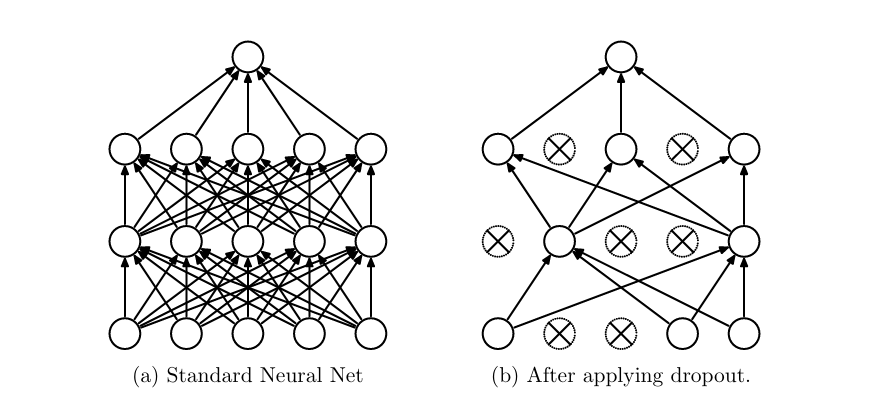
\includegraphics[width=1\linewidth]{dl/dropout.png}
        \caption{Visualizing dropout in a fully connected neural network}
        \label{fig:dropout}
    \end{figure}

    Why would we do this? Well, if a network is allowed to use all of its neurons all of the time, there is no guarantee that the network will \textit{effectively} use all the neurons. Perhaps due to a strange initial weight configuration, the random seed, or some other factor, the network will only use a very small subset of its available power. Many neurons will end up going essentially unused and their weights meaningless, despite the resources being allotted to train them. This consolidation of computation into a small portion of the network leads to much lower robustness. \break
    
    Here is an analogy: a 10-armed robot is trained to pick up an apple from a desk. The robot uses one of its arms at random, and only trains with that arm. Then during test time, we bind the arm the robot used the most. Since the robot has not learned how to use any of its other arms, it fails at a task it should very easily be able to do. Dropout is like forcing the robot to pretend it has lost a few arms each training example. It is then forced to use all of its arms, and gets good at picking up the apple with any of them. This robot is now much more robust when deployed into the real world, as small perturbations do not totally handicap it. \break

    One small detail is that once training time is over, all neurons have their weights scaled by 1 minus the dropout rate. Therefore, the expected distribution of values flowing from one layer to the next stays the same as it was during training time.
\end{flushleft}

\subsection{Batch Normalization}
\begin{flushleft}
    \large \textbf{Batchnorm:} Batchnorm, or batch normalization, is a very common technique used to regularize neural networks and improve training efficiency. Batchnorm can be thought of as an extra layer in a neural network with a few additional parameters. Essentially, before information flows from one layer to the next, the data is \textbf{normalized} across examples in the batch. Let's break this down. \break
    
    What is a \textbf{batch}? It is common to not just pass one example through a neural network at a time, but many. Groups of 64, 1024, 4096, etc. training examples are used at once before a backward pass is performed. Then what is \textbf{normalization}? Within this aforementioned batch, examples are mean-shifted by a mean $\mu$ and then divided by a standard deviation $\sigma$. This is normalization and it keeps the data centered around $(0,0)$ and evenly varied. In addition, these $\mu$ and $\sigma$ parameters are slightly adjusted for each new batch by taking a moving average through each previous batch. There are also additional ``scale and shift'' parameters represented by $\gamma$ and $\beta$ respectively. As the network sees more and more examples, the $\beta$ and $\gamma$ parameters are also slowly adjusted to find a scale and shift transformation to the normalized data that improves performance. This is shown in the following series of equations, where $x_i$ is a datapoint and $m$ is the number of datapoints in a batch. \break

    Estimating $\mu$ and $\sigma$ for a batch:
    $$\mu_{batch} = \frac{1}{m}\sum_{i=1}^m x_i$$
    $$\sigma_{batch} = \sqrt{\frac{1}{m}\sum_{i=1}^m (x_i - \mu_{batch})}$$
    Updating the moving average:
    $$\mu = \alpha \mu + (1-\alpha)\mu_{batch}$$
    $$\sigma = \alpha \sigma + (1-\alpha)\sigma_{batch}$$
    Normalize $x_i$ to $\Tilde{x}_i$ using the moving average:
    $$\Tilde{x}_i = \frac{x_i - \mu}{\sigma}$$
    Scale and shift before sending values to next layer:
    $$x_i^{output} = \gamma\Tilde{x}_i + \beta$$
    
    Mean-centered and evenly varied data allows gradient descent to descend the weights smoothly down to a optimal minimum. If two features input into a neural network were on wildly different scales (e.g. House price vs. number of bedrooms), then optimization becomes clunky. Making a large shift in weights is necessary to process highly varied housing prices, but this same shift negatively affects how the network processes the more tame ``number of bedrooms'' feature since more precise changes are needed. Normalization plus scale and shift removes this problem, and thus batchnorm helps greatly with a network's convergence.
\end{flushleft}

\begin{questionbox}
    \textbf{Synthesis Questions:}
    \begin{enumerate}
        \item In your own words, why does Dropout work?
        \item Why do you think a moving average of $\mu$ and $\sigma$ are useful for a network with batch normalization layers if there are many batches to process?
        \item Think of, or find online, a method of regularization within neural networks not discussed here. Write two to three sentences on how it works.
    \end{enumerate}
\end{questionbox}

\section{When to Use Deep Learning/Neural Networks}
\begin{flushleft}
    \large While we have shown the great power and ability of neural networks and deep learning, with all this power comes great cost. Neural networks are power-hungry, taking up significant computation power for all the processing they have to do. They are a powerful tool and should be used with caution and respect. As our i2 president once said, \textbf{don't use a bomb to cut a sandwich}. It is important to know when to use them. Deep learning models are useful for image, audio, and video classification or, in other cases, where non-linearity is necessary. Neural networks also require considerable amounts of data for a decent accuracy. Only use them when you have enough labeled data to properly train them on. In summary, while neural networks offer unmatched capabilities for complex tasks like image and audio classification, they are not always the most efficient tool. Sometimes a simpler model will get the job done while using half the resources. The key is understanding when their power is necessary and when a more lightweight solution will suffice. Always choose the right tool for the job.
\end{flushleft}

\section{Conclusion (DL)}
\begin{flushleft}
    \large This section covered the fundamental concepts of deep learning, with a heavy focus on neural networks. We also introduced important concepts like non-linearity and backpropagation. We closed with an overview of regularization techniques used in deep learning today. There is much more to deep learning we could not cover in this article. Neural networks especially are heavily used in many fields; either in larger deep learning architectures or as function approximators for some other goal. Understanding how they work and how to train them is critical to evaluating these systems. \break
\end{flushleft}